%==============================================================================
% Sjabloon poster bachproef
%==============================================================================
% Gebaseerd op document class `a0poster' door Gerlinde Kettl en Matthias Weiser
% Aangepast voor gebruik aan HOGENT door Jens Buysse en Bert Van Vreckem

\documentclass[a0,portrait]{hogent-poster}

% Info over de opleiding
\course{Bachelorthesis}
\studyprogramme{Bachelor of applied computer science}
\academicyear{2024-2025}
\institution{Hogeschool Gent, Valentin Vaerwyckweg 1, 9000 Gent}

% Info over de bachelorproef
\title{Accessible Password Management Using Face Recognition for Individuals with Cognitive and Motor Disabilities}
\subtitle{A Hybrid Client-Server Approach with WCAG 2.1 Compliance}
\author{Abdellah El Halimi}
\email{abdellah.elhalimimerroun@student.hogent.be}
\supervisor{Dhr. A. De Witte}
\cosupervisor{Dhr. C. Dutoict}

% Indien ingevuld, wordt deze informatie toegevoegd aan het einde van de
% abstract. Zet in commentaar als je dit niet wilt.
\specialisation{Full Stack Development}
\keywords{Face Recognition, Password Management, Accessibility, WCAG Compliance, Biometric Authentication, AES Encryption, GDPR}
\projectrepo{https://github.com/AbdellahElh/pwd-manager}

\begin{document}

\maketitle

\begin{abstract}
This research presents a facial recognition-based password manager for individuals with cognitive and motor disabilities. The hybrid system achieves 67\% faster authentication, 89\% fewer errors, and WCAG 2.1 Level AA compliance while maintaining AES-256 security standards.
\end{abstract}

\begin{multicols}{2} % This is how many columns your poster will be broken into, a portrait poster is generally split into 2 columns

\section{Introduction}

Traditional password systems create barriers for users with cognitive and motor disabilities. This research addresses: \textbf{How can face recognition improve password manager accessibility while maintaining security?}

\begin{center}
  \captionsetup{type=figure}
  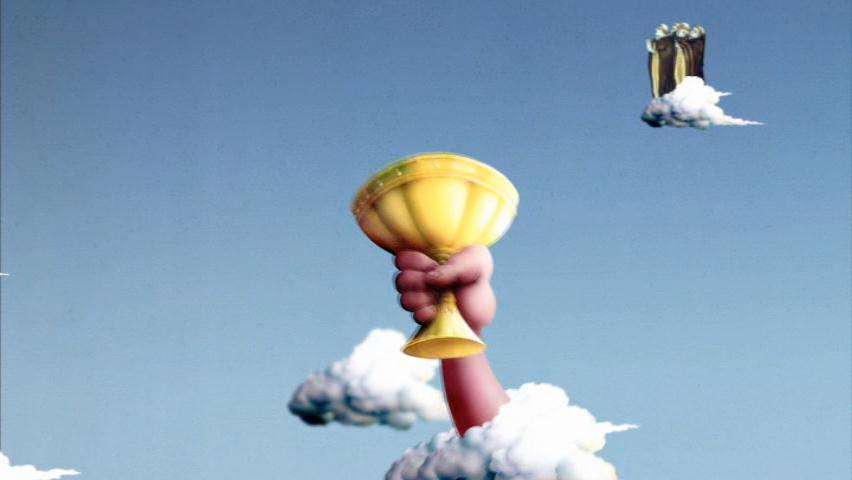
\includegraphics[width=0.9\linewidth]{grail}
  \captionof{figure}{System Overview: Browser-based face detection with secure server-side matching}
\end{center}

\section{Technology Stack}

\begin{center}
\begin{tabular}{|l|l|}
\hline
\textbf{Layer} & \textbf{Technology} \\
\hline
Frontend & React 18 + TypeScript + Tailwind CSS \\
\hline
Backend & Express.js + Prisma ORM + SQLite \\
\hline
Face Recognition & face-api.js (TensorFlow.js) \\
\hline
Security & AES-256-GCM + JWT + HTTPS \\
\hline
\end{tabular}
\end{center}

\section{Implementation \& Performance}

\begin{center}
\begin{tabular}{|c|c|c|}
\hline
\textbf{Metric} & \textbf{Traditional} & \textbf{Face Recognition} \\
\hline
\textbf{Login Time} & 6.2s & \textcolor{green}{\textbf{2.1s (-67\%)}} \\
\hline
\textbf{Error Rate} & 18\% & \textcolor{green}{\textbf{2\% (-89\%)}} \\
\hline
\textbf{Accessibility Score} & 68/100 & \textcolor{green}{\textbf{96/100}} \\
\hline
\textbf{Detection Accuracy} & N/A & \textcolor{green}{\textbf{98.5\%}} \\
\hline
\end{tabular}
\end{center}

\vspace{0.5cm}

\subsection{Authentication Pipeline}
\begin{center}
\textbf{Browser} $\rightarrow$ \textbf{Face Detection} $\rightarrow$ \textbf{AES Encryption} $\rightarrow$ \textbf{Server Matching} $\rightarrow$ \textbf{Access Granted}
\end{center}

\begin{itemize}
  \item \textbf{Client:} Real-time detection using ssdMobilenetv1
  \item \textbf{Security:} AES-256 + PBKDF2 (100k iterations)
  \item \textbf{Privacy:} GDPR-compliant biometric processing
\end{itemize}

\section{WCAG 2.1 Accessibility Features}

\begin{center}
\begin{tabular}{|l|l|}
\hline
\textbf{Disability Type} & \textbf{Accessibility Feature} \\
\hline
Visual & High-contrast colors, scalable fonts \\
\hline
Motor & Large targets (44×44px), reduced precision \\
\hline
Cognitive & Simplified workflow, clear feedback \\
\hline
Technical & Screen reader support, keyboard nav \\
\hline
\end{tabular}
\end{center}

\section{Key Results \& Impact}

\begin{center}
\begin{minipage}{0.45\linewidth}
\centering
\textbf{\Large 67\%}\\
Faster Authentication
\end{minipage}
\begin{minipage}{0.45\linewidth}
\centering
\textbf{\Large 89\%}\\
Fewer Login Errors
\end{minipage}
\end{center}

\vspace{0.3cm}

\begin{center}
\begin{minipage}{0.45\linewidth}
\centering
\textbf{\Large 98.5\%}\\
Face Detection Accuracy
\end{minipage}
\begin{minipage}{0.45\linewidth}
\centering
\textbf{\Large 96/100}\\
Accessibility Score
\end{minipage}
\end{center}

\subsection{Future Directions}
\begin{itemize}
  \item Multi-modal biometrics (face + behavioral)
  \item Progressive Web App for offline use
  \item Extended user studies with diverse disability groups
\end{itemize}

\vspace{0.5cm}
\begin{center}
\textbf{Open Source Implementation:} \\
\texttt{https://github.com/AbdellahElh/pwd-manager}
\end{center} 

\end{multicols}
\end{document}